\chapter{Introduction to Vehicle Congestion Control and Management System}
Traffic congestion at urban intersections represents one of the most pressing challenges in modern transportation infrastructure. Traditional fixed-timing traffic signals often fail to adapt to real-time traffic conditions, leading to inefficient vehicle flow and increased delays. This project presents an innovative solution that leverages Internet of Things (IoT) technologies and machine learning algorithms to create an intelligent traffic management system. The system integrates multiple sensing technologies including ultrasonic sensors for distance measurement, cameras for real-time vehicle detection, and advanced computer vision techniques to analyze traffic patterns and optimize signal timing dynamically.

\section[Introduction]{\textbf{Introduction}}

The Vehicle Congestion Control and Management System addresses the critical need for adaptive traffic control in busy urban intersections. Traffic congestion remains a significant challenge in urban areas, particularly where fixed-timing signals cause long delays and disrupt efficient vehicle flow. The relevance of this project stems from the growing urbanization and increasing vehicle density that demands smarter traffic management solutions.

This project introduces an intelligent traffic management system powered by IoT and machine learning technologies. The system employs a multi-sensor approach combining ultrasonic sensors for continuous vehicle distance measurement, infrared sensors for precise detection, and high-resolution cameras for comprehensive traffic analysis. The integration of these technologies enables real-time traffic density estimation and pattern recognition.

The historical evolution of traffic management systems has progressed from simple mechanical timers to electronic controllers, and now to intelligent systems capable of real-time adaptation. This project represents the next generation of traffic management, incorporating artificial intelligence and IoT connectivity to create a truly responsive traffic control system.

As in Figure \ref{fig:system_architecture} the Smart Traffic Management System Architecture utilizes a combination of ultrasonic and IR sensors to detect congestion levels, while urban sonic sensors and a YOLO model with OpenCV enable AI-based image processing for vehicle density detection. Data is collected and processed by an Arduino Mega and ESP8266, which then adjusts traffic signal durations accordingly. The system also features a website to display real-time traffic status, ensuring efficient traffic flow and congestion management. 
\begin{figure}[htb]
\centering
	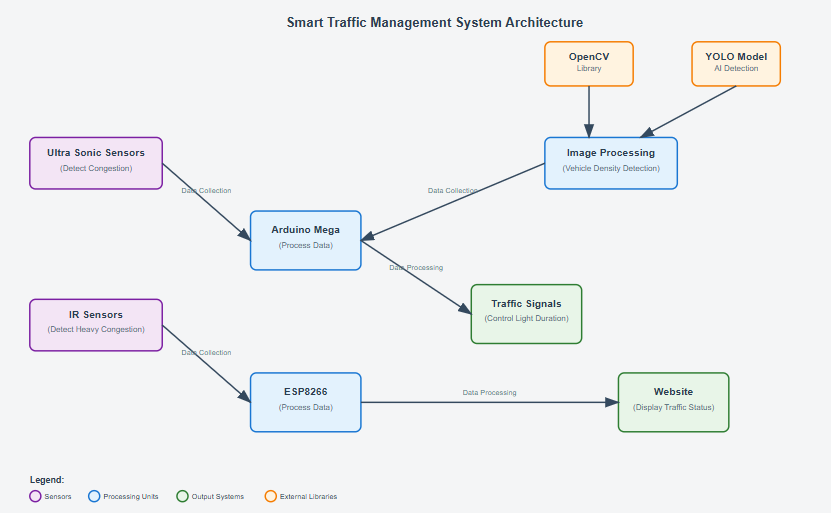
\includegraphics[scale=1]{Figures/system_architecture.png}	
	\caption{System Architecture of Intelligent Traffic Management System}
	\label{fig:system_architecture}
\end{figure}

\section[Motivation]{\textbf{Motivation}}

The motivation for selecting this project stems from the critical need to address urban traffic congestion and its associated problems. Traditional traffic management systems are inadequate for handling the dynamic nature of modern traffic patterns. The increasing vehicle density in urban areas, coupled with the need for emergency vehicle prioritization, creates an urgent requirement for intelligent traffic management solutions.

The challenges in current traffic management include inefficient fixed-timing systems, lack of real-time adaptability, poor emergency vehicle handling, and limited traffic data utilization. The relevance of this project lies in its potential to significantly improve traffic flow efficiency, reduce fuel consumption, minimize environmental impact, and enhance road safety through intelligent automation.

\section[Literature Review]{\textbf{Literature Review}}

The following table presents a concise review of key research papers related to traffic congestion control and emergency vehicle prioritization. The reviewed works focus on smart traffic systems, IoT-based management, swarm intelligence, and deep learning, with a focus on real-time implementation challenges and gaps in emergency prioritization and sensor integration.



\begin{table}[h!]
\begin{adjustbox}{width=\linewidth,left}
\begin{tabular}{|p{4cm}|p{3.5cm}|p{5.5cm}|p{4.5cm}|}
\hline
\textbf{Title} & \textbf{Authors} & \textbf{Summary} & \textbf{Research Gap} \\
\hline
Smart Traffic Management for Congestion Control and Emergency Vehicle Priority (2025) & IEEE Conference & Dynamic traffic signal adjustment and emergency vehicle prioritization & No predictive traffic flow modeling using historical data \\
\hline
A Swarm Algorithm for Collaborative Traffic (2025) & Jamal Toutouh, Enrique Alba & Distributed swarm intelligence for vehicle coordination & Lacks integration with real-time sensor or camera data \\
\hline
LSTM-Based Proactive Congestion Management (2024) & Aly Sabri Abdalla et al & Predicts congestion using LSTM & Does not prioritize emergency vehicles \\
\hline
Hybrid Deep Learning-Based Congestion Control (2024) & Alexandria Engineering Journal & Combines CNN, RNN, and optimization for smart city traffic control & High computational cost limits real-time use \\
\hline
Traffic Congestion Control with Emergency Awareness (2025) & IEEE Access & Genetic algorithms and reinforcement learning for congestion and emergency priority & Scalability under dense networks not evaluated \\
\hline
Congestion Control Mechanisms for IoV (2023) & Lakhdar Kamel Ouladdjedid & Survey of existing cooperative IoV congestion solutions & No real-time sensor or camera data usage \\
\hline
Smart Signaling with IoT and Sensors (2024) & G. Saranya et al & Uses sensors and AWS for real-time light control & No camera-based vehicle detection \\
\hline
Real-Time Traffic Control using IoT (2024) & S.M. Najrul Howlader et al & IR sensors adjust signals based on vehicle density & Unvalidated in real-world dynamic scenarios \\
\hline
\end{tabular}
\end{adjustbox}
\vspace{0.5em} % optional space between table and caption
\caption{Summary of Related Work and Research Gaps}
\label{tab:literature}
\end{table}


\section[Problem statement]{\textbf{Problem statement}}

Traditional traffic management systems rely on fixed-timing signals that cannot adapt to real-time traffic conditions, resulting in inefficient traffic flow, increased congestion, extended waiting times, and inadequate prioritization of emergency vehicles. There is a critical need for an intelligent traffic management system that can dynamically adjust signal timing based on real-time traffic density analysis, prioritize emergency vehicles, and provide traffic information to users for better route planning.

\section[Objectives]{\textbf{Objectives}}
The objectives of the project are
\begin{enumerate}
\item To design a smart traffic control system using ultrasonic sensors, IR sensors and image processing to detect vehicle density and dynamically manage signal timings
\item To implement machine learning algorithms that prioritize emergency vehicles like ambulances and adapt traffic signals based on real-time traffic patterns
\item To develop a web-based platform that provides real-time traffic updates, helping users identify congested routes and make informed travel decisions
\end{enumerate}

\section[Brief Methodology of the project]{\textbf{Brief Methodology of the project}}

The methodology for this project involves a multi-stage approach combining hardware sensor deployment, computer vision implementation, machine learning integration, and web-based dashboard development. The system architecture includes strategic placement of ultrasonic and IR sensors on key traffic lanes for real-time vehicle detection and density estimation.

The computer vision component utilizes high-resolution cameras with advanced object detection algorithms (YOLOv5/SSD) for vehicle classification and emergency vehicle identification. A supervised machine learning model, implemented using decision tree or random forest algorithms, analyzes historical and real-time data to predict traffic patterns and optimize signal timing.

The control system is built around ATmega2560 and ESP8266 microcontrollers, providing dynamic signal adjustment capabilities through GPIO-controlled relays. Emergency vehicle prioritization is achieved through camera-based object tracking and RF modules for immediate signal override. The web-based dashboard, developed using Flask/Django backend and HTML/CSS/JavaScript frontend, provides real-time traffic visualization and congestion monitoring.

\section[Assumptions made / Constraints of the project]{\textbf{Assumptions made / Constraints of the project}}

The project assumes adequate lighting conditions for camera-based vehicle detection and stable internet connectivity for IoT data transmission. The system is designed for standard four-way intersections with conventional traffic signal infrastructure. Weather conditions are assumed to be within normal operational parameters for electronic sensors.

Key constraints include the dependency on reliable power supply for continuous operation, the requirement for periodic sensor calibration and maintenance, and the need for initial training data collection for machine learning model development. The system's effectiveness is constrained by the accuracy of sensor readings and the quality of camera feed for computer vision processing.

\section[Organization of the report]{\textbf{Organization of the report}}

This report is organized as follows:
\begin{itemize}
\item Chapter 2 discusses the theory and fundamentals of traffic management systems, IoT sensor technologies, and machine learning algorithms for traffic optimization
\item Chapter 3 discusses the system design and architecture, including hardware component selection and software framework development
\item Chapter 4 discusses the implementation details of sensor integration, computer vision algorithms, and machine learning model development
\item Chapter 5 discusses the testing methodology, system performance evaluation, and experimental results analysis
\item Chapter 6 discusses the conclusions, project outcomes, future enhancements, and recommendations for deployment
\end{itemize}